\documentclass{amsart}
\usepackage{graphicx}
\usepackage{array}
\usepackage{moreverb}
\title{DRAFT: User Documentation for the STIDE software package}
\author{Julie Rehmeyer}
\date{\today}
\begin{document}
\maketitle 


\section{Software Purpose} \label{sec:intro}
STIDE stands for Sequence Time-Delay Embedding, and it implements the
time-delay embedding method of anomaly detection.  Its primary
function is to accept as input a time series (or a set of time
series), divide it into a set of fixed-length sequences, compare that
set of sequences with an existing database of fixed length sequences,
and report on the consistency of the time series with the existing
database.  It can also be used to created a database of fixed-length
sequences from scratch, or to add to a pre-existing database.

The STIDE software was originally developed by Steve Hofmeyr, a
graduate student in the Computer Science Department at the University
of New Mexico, as part of a research program that is applying ideas
from immunology to problems in computer security.  In particular,
STIDE was written to assist in detecting intrusions by identifying the
unusual sequences of system calls that may be created during an
attempted intrusion \cite{lightweight, ci, principles, self}. In this
context, the time series being considered consists of the system calls
made by a single process.  We first record the system calls made by a
process exibiting normal behavior (i.e., in non-exploited situations),
and then use STIDE to divide that continuous stream of system calls
into sequences of a given length and store them in a database.
Subsequently, when we want to know if another instance of the same
program has been attacked, we record the system calls the process has
generated and use STIDE to compare the resulting sequences of system
calls with the database of normal sequences.  A large number of
sequences created by the potentially attacked process that weren't
created by the uncompromised processes suggests that the process may
have been exploited.

In practice, because of limitations in available system call tracing
mechanisms, is far easier for us to record simultaneously the system
calls generated by several processes that are running at the same
time.  STIDE is designed to handle this sort of situation.  It can
simultaneously process multiple interwoven time series by requiring
that each element in the input stream be preceded by an identifier to
specify which series it comes from.  In our work, that identifier is
the process ID.

The simplest way that STIDE can analyze information about the
consistency of new data with an existing database is to report the
number of anomolous sequences, i.e., the number of sequences in the
input which do not exist in the database.

It can also report the minimum Hamming distance \cite{lightweight}.
Given a sequence from the data stream and a sequence from the
database, we can compute the number of entries that are different
between the two sequences and get the Hamming distance between those
two sequences.  The minimum of the Hamming distances between the input
sequence and all of the sequences from the database is the minimum
Hamming distance for the input sequence.

The final option is that it can report a ``locality frame count''
\cite{ci}.  When a process is exploited, there may be a short period
of time (a locality) when the percentage of anomolous sequences is
much higher.  Although ten anomalies over the course of a long
run may not be cause for concern, ten anomalies within thirty
sequences might be.  Thus it can be useful to observe how many
anomalies there are {\it locally}.  The number of sequences that are
considered to be ``local'' to one another is called the size of the
locality frame.  In this mode, STIDE reports the largest number of
anomalies it finds within any locality frame.

An additional advantage of calculating locality frame counts is that
it provides an ``on-line'' measure.  Ultimately, we are interested in a
system which would detect intrusions as the system is running.
Because locality frame counts are calculated locally, one can
immediately be notified when an intrusion may be occurring.

\section{Input Data Format} \label{sec:input}
The input data consists of the time series to be analyzed.  It is read
from standard input.  It is expected to be a series of pairs of
positive integers, one pair per line, where the first integer
identifies the data stream and the second integer is the element of
the data stream.  The end of the data stream can either be designated
by the end of the file or by an occurrence of the number $-1$ as a
stream identifier.  In our work, the stream identifier is the process
identification number (PID), and the elements of the data stream are
system call numbers.  

The following is a small example of an input file, tracking three
processes, with PID's 744, 1069 and 9.

\vspace{.15in}
\begin{tabular}{l l}
744  & 24   \\
744  & 13   \\
1069 & 4    \\
1069 & 24   \\
1069 & 4    \\
744  & 5    \\
9    & 24   \\
1069 & 13   \\
744  & 81   \\
9    & 13   \\
9    & 2    \\
1069 & 5    \\
1069  & 18  \\
-1 
\end{tabular}
\vspace{.15in}

If the number $-1$ occurs as a data element, STIDE interprets that as
a missing data element.  It does not form any sequences going through
that data element.  It clears the sequence and starts from scratch.

For example, suppose that the sequence length is 3 and the input is as
follows:
\nopagebreak
\vspace{5pt}
\begin{tabular}{l l}
220  &  14  \\
220  &  185 \\
220  &  20  \\
220  &  -1  \\
220  &  2   \\
220  &  20  \\
220  &  3   \\
220  &  2  \\
-1 
\end{tabular}
\vspace{.15in}

STIDE would  derive three sequences from this input: 14, 185, 20; 2,
20, 3; and 20, 3, 2.

\section{Configuration Options}
There are a number of options which affect STIDE's behavior.  Every
option has a default value.  The values may be changed through command
line arguments or through a configuration file.  Values set by the
configuration file override default values and values set by the
command line override those set by either the configuration file or
the defaults.  The following options are available:

\vspace{.2in}
\setlength{\extrarowheight}{3pt}

\begin{tabular}{l|l|l|l}

\vspace{-3pt}
Short &&& \\
Name & Long name & Legitimate Values & Default Value \\ 
\hline 

{\tt a}   & {\tt add\_to\_db}       & on or off         & off \\ 
{\tt c}   & {\tt config\_name}      & filenames         & stide.config \\ 
{\tt d}   & {\tt db\_name}          & filenames         & default.db \\ 
{\tt f}   & {\tt lf\_size}          & 1 -- 999          & 1     \\ 
{\tt g}   & {\tt output\_graph}     & on or off         & off   \\ 
{\tt l}   & {\tt seq\_len}          & 1 -- 199          & 6     \\ 
{\tt p}   & {\tt pair\_offset}      & integers          & 0     \\ 
{\tt s}   & {\tt write\_db\_stats}  & on or off         & off   \\ 
{\tt v}   & {\tt verbose}           & on or off         & off   \\ 
{\tt V}   & {\tt very\_verbose}     & on or off         & off   \\ 
{\tt hd}  & {\tt compute\_hdist}    & on or off         & off   \\ 
{\tt me}  & {\tt max\_elements}     & 1 -- 999          & 500   \\ 
{\tt ms}  & {\tt max\_streams}      & 1 -- 999          & 100   \\ 
{\tt aof} & {\tt add\_output\_format} & see below       & see below \\ 
{\tt cof} & {\tt compare\_output\_format} & see below   & see below \\ 

\end{tabular}

\vspace{.2in}

\subsection{Descriptions of Options}

\subsubsection{Option {\tt add\_to\_db} }
 
This flag indicates that you want the input data to be added to the
database.  If there is no pre-existing database, it indicates that you
want to create a new database from the input data.  Note that you
cannot simultaneously compare data and add it to the database.  If
this switch is off, STIDE compares the input data with the database
without adding it.

\subsubsection{Option {\tt{config\_name}}}
This is the name of the configuration file to be used.  See
Section~\ref{subsec:config} for more information about the
configuration file.

\subsubsection{Option {\tt db\_name}}
This is the name of an existing database or the name under which to
store a new database that will be created from the input data.

\subsubsection{Option {\tt lf\_size}}
This is the size of the locality frame (see Section~\ref{sec:intro}
for an explanation of locality frame count).  The value 1 effectively
turns off locality frames.

\subsubsection{Option {\tt output\_graph}}
This causes STIDE to create a file {\tt db\_name.dot} containing a
graph of the entire database forest formatted as input for the program
Dot.  Running Dot on the file translates it into PostScript format.
The result is a graphical image of the database.

\subsubsection{Option {\tt seq\_len}}
A database stores trees of sequences of a set length.  When building a
new database, the length of the sequences to be stored is set with
{\tt seq\_len}.  When adding to or comparing with an existing
database, one must use the same sequence length that was used when the
database was generated.  In those situations, STIDE will automatically
figure out the correct sequence length and use it regardless of the
user specification or the default.\footnote{STIDE can do this for
  revision 1 databases only.  STIDE can still process old-style
  databases, but cannot implement this feature.  STIDE recognizes
  revision 1 databases by their initial line: {\tt \#DBrev: 1 } and the
  following line: {\tt \#DBseq\_len: }  followed by an integer giving
  the sequence length.  When STIDE processes an old-style database, it
  converts it to a revision 1 database if it is in {\tt add\_to\_db}
  mode.} 

\subsubsection{Option {\tt pair\_offset}} \label{subsubsec:po}
In {\tt verbose} or {\tt very\_verbose} modes, STIDE reports on
particular sequences of interest (see Sections \ref{subsubsec:verbose}
and \ref{subsubsec:very-verbose}).  One of the pieces of information
one might be interested in is where a particular sequence occurs in
the input.  Recall that the input data is a stream of pairs (stream
number, element number), and each element in the sequence being
considered came from one of those input pairs.  STIDE reports on where
the sequence occurred in the input by reporting the pair number of the
last element of the sequence.

These numbers may be offset by a fixed amount by setting {\tt
pair\_offset}. 

\subsubsection{Option {\tt write\_db\_stats}}
This flag causes STIDE to print out statistics on the database.  The
statistics it will print are the number of nodes in the database, the
number of unique sequences, the number of branches, and the average
database branch factor.  See Section~\ref{sec:output} for more
information.

\subsubsection{Option {\tt verbose}} \label{subsubsec:verbose}
When adding to the database in {\tt verbose} mode, STIDE will print
information about each new sequence being added to the database, where
the precise information is specified by the {\tt add\_output\_format}
parameter (see Section~\ref{subsubsec:aof}).  When comparing the input
data with an existing database in {\tt verbose }mode, it will print
information about each sequence that is itself a miss or whose
locality frame contains a miss, where the precise information is
specified by the {\tt compare\_output\_format} parameter (see
Section~\ref{subsubsec:cof}).  In either case, when adding or
comparing, STIDE will first print out a header with a list of the names
of the variables being printed.

\subsubsection{Option {\tt very\_verbose}} \label{subsubsec:very-verbose}
In {\tt very\_verbose} mode, STIDE will print out the information specified
by {\tt add\_output\_format} or {\tt compare\_output\_format} for each sequence
encountered in the input data, regardless of whether the sequence is
new.  As in {\tt verbose} mode, STIDE will first print out a header
with a list of the names of the variables being printed.

\subsubsection{Option {\tt compute\_hdist}}
This switch causes the Hamming distance \cite{lightweight} to be
computed (see Section~\ref{sec:intro} for an explanation of Hamming
distance).
  
\subsubsection{Option {\tt max\_elements}}
This is the maximum number of unique data elements that STIDE might
encounter in the input data.

\subsubsection{Option {\tt max\_streams}}
This is the maximum number of different data streams that STIDE might
encounter in the input data.

\subsubsection{Option {\tt add\_output\_format}} \label{subsubsec:aof}

When adding to the database in {\tt verbose} or {\tt very\_verbose}
modes, STIDE will print the {\tt add\_output\_format} string for every
sequence of interest (see Sections \ref{subsubsec:verbose} and
\ref{subsubsec:very-verbose}).  Substitutions are made for control
characters as follows:

\vspace{.15in}

\begin{tabular}{c|l}
\vspace{-4pt}
Control \\ Char &  Meaning \\ \hline
       \%s  & Stream Identification Number \\
       \%d  & Database Size  \\
\vspace{-4pt}
       \%p  & Pair number of last data element of \\
            & sequence in the whole input stream  \\
\vspace{-4pt}
       \%i  & Pair number of last data element of    \\
            & sequence in its particular data stream \\
       \verb+\+t & Tab    \\
       \verb+\+n & Newline    \\
\end{tabular}

\vspace{.15in}

See section \ref{subsubsec:po} for more information about the meaning
of the \%p and \%i control characters.

The default value of {\tt add\_output\_format} is:

\vspace{5pt}

\verb+"DB Size: %d\tStream: %s\tPair Number: %p\n"+
  
\subsubsection{Option {\tt compare\_output\_format}} \label{subsubsec:cof}
When comparing data in {\tt verbose} mode, STIDE will print the 
{\tt compare\_output\_format} string for every sequence which is
itself an anomaly or whose locality frame conatins an anomaly.  In
{\tt very\_verbose} mode, STIDE will print the string indicated for
{\it every} sequence, regardless of whether it is an anomaly.
Substitutions are made for control characters as follows:

\vspace{.15in}

\begin{tabular}{c|l}
\vspace{-4pt}
Control \\ Char &  Meaning \\ \hline
       \%s  & Stream Identification Number \\
\vspace{-4pt}
       \%p  & Pair number of last data element of \\
            & sequence in the whole input stream \\
\vspace{-4pt}
       \%i  & Pair number of last data element of \\
            & sequence in its particular data stream  \\
       \%a  & 1 if this sequence is an anomaly, 0 otherwise  \\
       \%c  & locality frame count of this sequence  \\
       \%h  & Hamming distance \\
       \verb+\+t & Tab    \\
       \verb+\+n & Newline    \\
\end{tabular}

\vspace{.15in}

See section \ref{subsubsec:po} for more information about the meaning
of the \%p and \%i control characters.

The default value of {\tt compare\_output\_format} is:

\vspace{5pt}

\verb+"Pair Number: %p\tStream Number: %s\n"+

\subsection{Command-Line Arguments}
All parameters may be set using the command line, in one of two ways.
The short name may be used, preceeded by a hyphen and followed by a
value (if appropriate).  The long name may also be used, but it must
be preceeded by {\it two} hyphens and followed by a value (if
appropriate).  Values set by the command line override those set in
any other way.

Switches which are simply turned on or off need not be followed by a
value.  Parameters may be set in any order. There must be space
between the parameter name and the value.  Flags may not be combined.

STIDE expects the input data to come from standard input.

\subsubsection{Examples}

To use STIDE to create a database called ``our\_data.db'' from the
input file ``input1.dat'' with sequences of length 10, using the
default configuration file name, in verbose mode, with ouput format
``\verb+%p\t%s\t%d\n+'',  one could type:

\vspace{5pt}

\begin{verbatim}
stide -d our_data.db -a -l 10 -v -aof "%p\t%s\t%d\n" < input1.dat
\end{verbatim}

\vspace{5pt}

To add the data from the file ``input2.dat'' to that database, using
the same configuration file, not in verbose mode, and to create a
graph in dot format, one could type:

\vspace{5pt}

\begin{verbatim}
stide -d our_data.db --output_graph --add_to_db -l 10 < input2.dat
\end{verbatim}

\vspace{5pt}

Then to compare the data in file ``input3.dat'' to the database and
have the results reported using locality frame counts with locality
frame size 20, using the configuration file ``run3.config'', one would
type:

\vspace{5pt}

\begin{verbatim}
stide -d our_data.db -f 20 -l 10 -c run3.config < input3.dat
\end{verbatim}

\vspace{5pt}

\subsection{Configuration File} \label{subsec:config}
All parameters may be set using a configuration file.  The first line
of a configuration file must be:\footnote{Old-style configuration
  files lack this line.  STIDE will assume that configuration files
  that lack this line are old-style, and will try to parse them
  accordingly, issuing a warning to the user.}

\vspace{5pt}

\begin{verbatim}
#ConfigFileRev: 1
\end{verbatim}

\vspace{5pt}

After the first line, lines may be commented out using a ``\#'' sign.
Each parameter is set on its own line, using the long name followed by
a colon, followed by the value.  Lines may be continued by putting a
backslash as the last character of the line.  White space at the
beginning of lines will be ignored.  Parameters which are simple
switches may be set with the value ``on'' or ``off'', or with no value
at all (which will turn them on).

Configuration file values override default values and are overriden
by command-line values.

\subsubsection{Example}

The following is a  sample configuration file:

\vspace{.15in}

\begin{boxedverbatim}

# ConfigFileRev: 1
# Sample STIDE configuration file containing default values.

 db_name: default.db     # name of database
 seq_len: 6              # length of sequences
 max_elements: 1000      # maximum number of unique elements 
			 # in input 
 max_streams: 500        # maximum number of unique streams 
 			 # in input  
 pair_offset: 0          # offset for pair number count
 add_output_format:  \
         "DB Size: %d\tStream: %s\tPair Number: %p\n"
 compare_output_format:  \
         "Pair Number: %p\tStream Number: %s\n"
 lf_size: 1              # 1 causes locality frame counts not
                         # to be computed 
 add_to_db: off          # Add this data to the database, or, 
                         # if there is no database, create a 
                         # new one -- do not do comparisons
 output_graph: off       # Outputs graphing information in Dot
                         # format 
 compute_hdist: off      # Compute Hamming distances
 write_db_stats: off     # At end, print out statistics about 
 			 # database
 verbose: off            # Verbose mode
 very_verbose: off       # Very verbose mode

\end{boxedverbatim}

\section{Output Data} \label{sec:output}
For every run, STIDE will first output the final configuration data
assembled from the defaults, the configuration file and the
command-line arguments, in a format which could be used as a
configuration file. The subsequent output depends on whether STIDE was
adding to the database or making comparisons.

\subsection{Output Data About Comparisons}

If you have run the program to compare sequences, at the end STIDE
will print out the number of different streams in the input, the total
number of pairs read from the input, the total number of sequences
read from the input, the number of sequences that were anomalous, and
the percentage of sequences that were anomalous.  If locality frame
counts were being computed, STIDE reports the maximum locality frame
count encountered in any stream, and if Hamming distances were being
computed, STIDE reports the largest minimum Hamming distance of any
sequence in any stream.

If the {\tt verbose} switch was on and the {\tt
  compare\_output\_format} parameter is set appropriately, STIDE will
print out information about each sequence which is either itself an
anomaly or whose locality frame contains an anomaly (if locality
frames are being computed).  If the {\tt very\_verbose} switch was on
and the {\tt compare\_output\_format} parameter is set appropriately,
STIDE will print out information about each sequence, regardless of
whether it is an anomaly.  The precise information to be output is
specified by the user in {\tt compare\_output\_format}.  See Section
\ref{subsubsec:cof} for details on what information {\tt
  compare\_output\_format} may request.

\subsection{Output Data About The Database}

If you are adding to the database, STIDE will not print out any
information automatically (beyond the configuration information).
However, one can get further information about the growth of the
database by turning on {\tt verbose} or {\tt very\_verbose} modes, and
one can get information about the shape and complexity of a database
using the {\tt write\_db\_stats} switch.

\subsubsection{Database Growth Information}

In {\tt verbose} mode, STIDE will print out information on each new
sequence which is added to the database.  In {\tt very\_verbose} mode,
STIDE will print out information on each sequence read in, regardless
of whether it is new.  The information that STIDE produces is
determined by the {\tt add\_output\_format} parameter.  See Section
\ref{subsubsec:aof} for details on what information may be requested.

\subsubsection{Database Statistics}

The {\tt write\_db\_stats} switch causes STIDE to print out
information about the shape and complexity of the database.  The {\tt
write\_db\_stats} switch may be used either when adding to the
database or when making comparisons.

The sequences are stored as forests (groups of trees).  Each path down
each tree represents a sequence that STIDE has encountered.  STIDE can
compute the number of nodes on the trees, the number of leaves (leaves
are the ends of the trees, i.e., the last element in a sequence), the
number of branches, and the average branch factor, which is the number
of branches divided by the difference between the number of nodes and
the number of sequences.

For example, consider the sequences derived from the first sample input file in
Section~\ref{sec:input}:
\nopagebreak
\vspace{5pt}

\begin{tabular}{c}
24, 13, 5  \\
13, 5, 81  \\
4, 24, 4 \\
24, 4, 13 \\
4, 13, 5  \\
13, 5, 18 \\
24, 13, 2  \\
\end{tabular}

\vspace{.15in}

We can represent those sequences by the forest:

\vspace{.15in}

\begin{picture}(350, 80)
\put(40,0){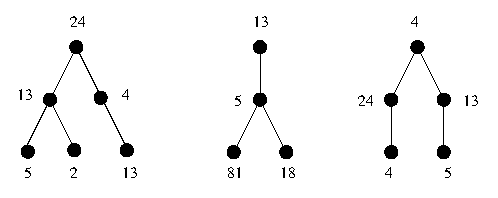
\includegraphics{graphic1.eps}}
\end{picture}

\vspace{.15in}

In this database, the number of nodes is 15, the number of leaves is
7, and the number of branches is 12.  There are 7 unique sequences.
The average branch factor is $12 / (15 - 7) = 1.5$.

\begin{thebibliography}{99}
  
\bibitem{lightweight} S. Hofmeyr, S. Forrest, and A. Somayaji
  ``Lightweight intrusion detection for networked operating systems.''
  Submitted to {\em Journal of Computer Security} (July, 1997).
  
\bibitem{ci} S. Forrest, S. Hofmeyr, and A. Somayaji ``Computer
  immunology'' {\em Communications of the ACM} Vol. 40, No. 10, pp.
  88-96 (1997).
  
\bibitem{principles} A. Somayaji, S. Hofmeyr, and S. Forrest
  ``Principles of a Computer Immune System.''  New Security Paradigms
  Workshop (presented September, 1997).
  
\bibitem{self} S. Forrest, S.~A. Hofmeyr, A. Somayaji, and T.~A.
  Longstaff ``A sense of self for Unix processes.''  In Proceedings of
  the 1996 IEEE Symposium on Computer Security and Privacy, IEEE
  Computer Society Press, Los Alamitos, CA, pp. 120-128 (1996).
\end{thebibliography}

\end{document}